\subsection{Evolutionäre Algorithmen} \label{subsec:Grundlagen_EvolutionäreAlgorithmen}

Evolutionäre Algorithmen stellen im Bereich der Metaheuristiken und in künstlichen Intelligenzen einen großen Forschungsbereich dar. Die Basis der evolutionären Algorithmen führt auf Charles R. Darwin zurück, welcher als Vater der Evolutionstheorie bekannt ist. Lebewesen, die sich innerhalb ihrer Umgebung am besten anpassen können setzten sich durch und übergeben ihren Nachfahren nützliche überlebenswichtige Eigenschaften. \cite[vgl.][S. 115]{siarry_metaheuristics_2016} \\

Der Oberbegriff \glqq evolutionäre Algorithmen\grqq{} fasst die Basis der Evolutionstheorie auf und wird genutzt, um Probleme in den Ingenieurswissenschaften zu lösen. Evolutionäre Strategien wurden in den 60er Jahren von Schwefel und Rechenberg vorgestellt und nutzen die Genetik, um Optimierungsprobleme mit kontinuierlichen Variablen zu lösen. Mitte der 60er wurde von Fogel et al. die evolutionäre Programmierung vorgestellt. Die genetischen Algorithmen, vorgestellt in 1975 von Holland, als Forschungsfeld populär geworden in 1989 von Goldberg, tragen dazu bei, die Funktionsweisen von selbstanpassenden Systemen zu verstehen. Genetische Algorithmen werden zudem als Metaheuristik genutzt, um Lösungen für Optimierungsprobleme zu finden. \cite[vgl.][S. 116]{siarry_metaheuristics_2016} \\
Diese Arbeit beschränkt sich somit auf die \acp{GA}, eine Untermenge der evolutionären Algorithmen. 

\begin{figure}[H]
    \centering
    \noindent\makebox[\textwidth]{%
    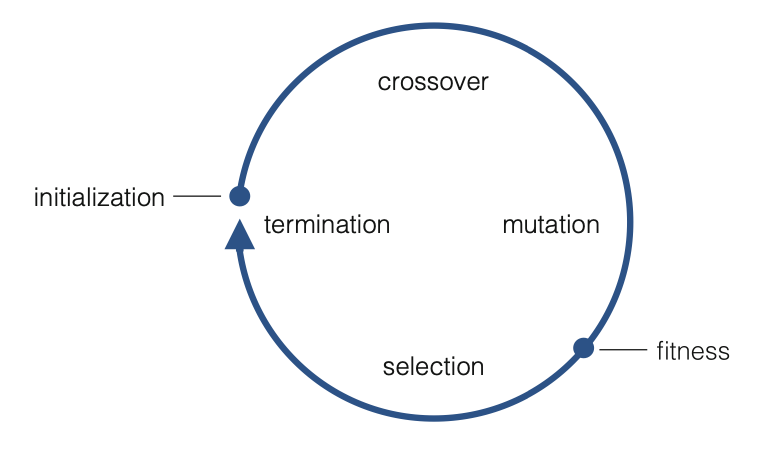
\includegraphics[width=0.57\textwidth]{assets/img/02_Grundlagen/CircleGA.png}
    }
    \caption{Kreislauf eines \acf{GA}} 
    \label{img:ga_cirlce}
    \source{\cite[][S. 5]{kramer_genetic_2017} }
\end{figure}

Abbildung \ref{img:ga_cirlce} zeigt den Kreislauf eines genetischen Algorithmus, basierend auf der natürlichen Evolution. Zu Beginn wird eine Population generiert, was zufällig oder manuell (z. B. über heuristische Regeln) geschehen kann. Über eine Crossover-Operation werden zwei oder mehrere Eltern rekombiniert, um so ein oder mehrere Nachfahren zu erzeugen. Zudem sind die Nachfahren nach dem Crossover gemäß einer Mutations-Operation mutiert. In der Selektionsphase werden entsprechend einer Regel die besten Ergebnisse gemäß ihres Fitnesswertes ausgewählt. Der Algorithmus läuft solange durch, bis das beliebige Terminierungskriterium erfüllt wurde. \cite[vgl.][S. 5]{kramer_genetic_2017} 

\begin{lstlisting}[caption={Genetic Algorithm (Quelle: \cite[vgl.][S. 119]{siarry_metaheuristics_2016}}), label=lst:ga, mathescape=truexinputencoding={utf8}, extendedchars=false, escapeinside=``]
Select size of parents $\mu$;
Select size of offsprings $\lambda$;
init population $P$ with $\mu$ individuals; 
fitness evaluation $\forall i \in P: f(i)$ of population $P$; 
while stopping criteria not satisfied do
    for i in range(0, $\lambda$) do
        select parents $\kappa$ from population;
        $x \leftarrow$ crossover $\kappa$;
        $x \leftarrow$ mutate $x$;
        fitness evaluation $f(x)$; 
    end
    selection of $\mu$ individuals for next generation population $P$
end
return the best individual;
\end{lstlisting}

Listing \ref{lst:ga} stellt den Pseudocode des Algorithmus dar. $\mu$ steht für die Anzahl der Eltern, $\lambda$ für die der Nachkommen \cite[vgl.][S. 119]{siarry_metaheuristics_2016}. Der aufgeführte Algorithmus ist generisch gehalten, da für die Crossover-, Mutations- und Selektionsoperationen \cite[vgl.][S. 118]{siarry_metaheuristics_2016} verschiedene Strategien je nach Problemart existieren. Außerdem für das Problem angeschnitten ist die Repräsentation eines Individuums. Diese kann beispielsweise eine binäre \cite[vgl.][S. 137]{siarry_metaheuristics_2016}, reale \cite[vgl.][S. 140]{siarry_metaheuristics_2016} oder beliebige diskrete \cite[vgl.][S. 149]{siarry_metaheuristics_2016} Struktur aufweisen. \\

Bei der Crossover-Operation findet eine Rekombination zweier oder mehrerer (Eltern-)Individuuen $\mu_1, \mu_2$ statt. Eine einfache Crossover-Operation für kontinuierliche Variablen ist die Verwendung eines Arithmetic Crossover. Hierbei wird das arithmetische Mittel aus den Eltern berechnet, welches der Nachfahre darstellt. Bei zwei Eltern mit $\mu_1 = (1, 2, 3)$ und $\mu_2 = (5, 4, 3)$ wäre der Nachfahre $\lambda_1 = (3, 3, 3)$. \cite[vgl.][S. 13]{kramer_genetic_2017}\\

Im Hinblick auf die Masterthesis stehen beim \ac{GA} die diskreten Strukturen im Vordergrund. Eine diskrete Struktur bei Individuen könnten Reihenfolgen darstellen, in welcher Sequenzen nur einmalig vorhanden sein können\cite[vgl.][S. 151]{siarry_metaheuristics_2016}, oder ggf. mit Vorgängeraktivitäten verknüpft sind, wie dies bei Aktivitätslisten beim (M)\ac{rcpsp} der Fall ist (vgl. Abschnitt \ref{subsec:SGS_Aktivitaeten}). \\

\begin{figure}[H]
    \centering
    \noindent\makebox[\textwidth]{%
    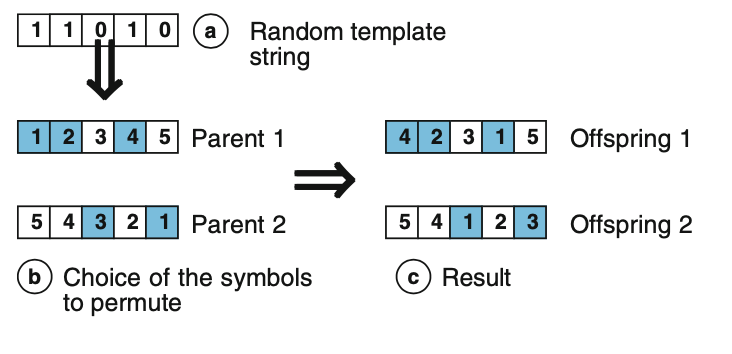
\includegraphics[width=0.70\textwidth]{assets/img/02_Grundlagen/GA_UniformOrderCrossover.png}
    }
    \caption{Uniform Order-Based Crossover} 
    \label{img:ga_uniformcrossover}
    \source{\cite[][S. 151]{siarry_metaheuristics_2016} }
\end{figure}

Abbildung \ref{img:ga_uniformcrossover} stellt einen Uniform Order-Based Crossover dar, welcher sich in drei Phasen einteilen lässt und sich auf zwei Eltern-Individuen anwenden lässt. Zunächst wird ein zufällig generiertes binäres Template verwendet, welches die Positionen der Sequenzen der Eltern die zur Rekombination verwendet wird, vormerkt. Im Beispiel sind bei Parent 1 die Sequenzen 1, 2 und 4, bei Parent 2 die Sequenzen 3 und 1 vorgemerkt. Das Vormerken gibt an, dass die Elemente gemäß der Reihenfolge des anderen Elternteils permutiert werden können. \cite[vgl.][S. 151]{siarry_metaheuristics_2016} \\ 

% Ein weiterer Operator, welcher bspw. konkret für das \ac{rcpsp} eingesetzt wird stellt der Two-Point Operator dar. Hierbei werden zunächst zwei zufällige Punkte $q1, q2$ innerhalb der Aktivitäten selektiert. Es gilt $1 \leq q1 < q1 \leq J$.\\

Bei einer Mutation-Operation werden kleine, zufällige Änderungen an einem (Nach-kommen-)Individuum $\lambda_1$ vorgenommen. Die Mutation dient als Möglichkeit, den Suchraum weiter außerhalb der Population $P$ zu erkunden. Bei kontinuierlichen Variablen stellt die Gaussian Mutation eine etablierte Operation dar. Hierbei wird eine zufällige reale Zahl von der Normalfunktion $\mathcal{N}(0, 1)$ generiert. Sei $\sigma$ die Mutationsrate, dann wäre ein Nachkommen $\lambda_1$ über $\lambda_1' = \lambda_1 \cdot \mathcal{N}(0, 1)$ mutiert. \cite[vgl.][S. 13 f.]{kramer_genetic_2017}\\

Die Mutation durch Austausche-Operation stellt eine mögliche Variante für diskrete Variablen mit Reihenfolgenbeziehungen dar. Diese wählt zwei Sequenzen innerhalb eines Individuums $\lambda_1$ aus und vertauscht diese miteinander, wenn die Beschränkungen gemäß des Problems eingehalten werden können. \cite[vgl.][S. 154]{siarry_metaheuristics_2016}\\

Eine weitere Komponente von genetischen Algorithmen stellt die Fitness eines Individuums dar. Die Fitness eines Individuums sagt aus, wie gut die Qualität hinter dem Individuum ist \cite[][S. 16 f.]{kramer_genetic_2017}. Dies kann im Fall von Optimierungsproblemen die Kostenfunktion (z. B. die Projektdauer beim \ac{rcpsp}) sein. Zudem müssen Aspekte, wie Multi-Objectives oder Bestrafen durch Verletzungen von Beschränkungen über die Fitness-Funktion abgedeckt werden \cite[vgl.][S. 16 f.]{kramer_genetic_2017}. \\

Die Selektion stellt im generischen \ac{GA} die letzte Operation einer Iteration bzw. der Generation dar und wählt die Individuen für die Folge-Population aus. Für die Auswahl der Individuen zur nächsten Generation stehen unterschiedliche Varianten zur Verfügung. Eine Variante stellt ein $(\mu, \lambda)$-\ac{GA} dar. Diese entspricht der Komma-Selektion, welche die $\mu$ besten Lösungen aus den $\lambda$ erzeugten Nachfahren der aktuellen Generation selektiert. $(\mu+\lambda)$-\ac{GA} verwendet die Plus-Selektion, d.h. die $\mu$ besten Lösungen sowohl aus den $\lambda$ erzeugten Nachfahren als auch die Eltern $\mu$ der aktuellen Generation werden selektiert. \cite[vgl.][S. 16 f.]{kramer_genetic_2017}. \\

Die Terminierung eines \ac{GA} geschieht z. B. über das Durchlaufen einer festen Anzahl an Generationen, der CPU-Zeit, das Erreichen eines vorgegebenen Fitnesswertes oder nach Feststellung einer Sättigung et cetera. \cite[vgl.][S. 17 f.]{kramer_genetic_2017}.